\documentclass{ml}

\begin{document}
\maketitle{Rest-It}{Sun, 09 Jun 2013 23:59}{Mareike Picklum}{z3446393}{Johan Klokkhammer Helsing}{z3432903}

%------------------------------------------------------------------------------

\section{Introduction}
\label{intro}
The project \textit{Rest-It} is an implementation of a reinforcement learner for the popular puzzle game Tetris. 
The core idea of the game is to place Tetronimoes (pieces consisting of four connected cells) in the way that the complete as many lines as possible in a 10 columns by 20 rows playing field.
Each completed line is removed from the field and the cells above are moved one cell down.
Removing a line adds one to the players score.
Tetris is a common benchmark problem for testing machine learning algorithms, as it uses comparably simple rules although it requires complex strategies to perform well. 

In \nameref{relatedwork} we will give a short overview about existing reinforcement learning approaches for Tetris and give information about what our project is based on and influenced by.
We will then describe the algorithms we implemented in \nameref{method} and present our results in \nameref{results}.
We will give a short summary and wrap up the results in \nameref{conclusions}.

%------------------------------------------------------------------------------

\section{Related work}
\label{relatedwork}
There are different approaches for tetris learners. 
\cite{szepesvari2010algorithms} describes different reinforcement learning algorithms and their core ideas and discusses their theoretical  limitations. \\
\cite{szita2006learning} apply noise to improve the cross-entropy method by preventing it from early convergence and achieve a policy that outperforms previous algorithms by almost two orders of magnitude.\\
\cite{carr2005applying} introduces reinforcement learning for Tetris and introduces the Formal Tetris Specification by \cite{faheytetris}.\\
\cite{gross2008learningto} investigate the idea of temporal difference learning applied to the Tetris problem and train agent using an $\varepsilon$-greedy policy. 

Our code is based on an open source Qt Project\footnote{\href{https://qt-project.org/doc/qt-4.8/widgets-tetrix.html}{Qt Project}} implementation of tetris. \\
The core idea for the reinforcement learning algorithm we use is described by \cite{zucker2009learning}, which will be investigated in more detail in \nameref{method}.

%------------------------------------------------------------------------------

\section{Method}
\label{method}

Following the remarks in \cite{zucker2009learning}, we first defined the properties of the game needed to calculate the quality.
According to the common Tetris rules, a player can rotate, move and drop a Tetronimo. As it is an easy representation, we describe an action $u$ as a position and rotation of a piece: $u = (p,r)$. The state $x$ of the game consists of the current board occupancy, the current Tetronimo to be played, and the next Tetronimo to be spawned (in time step $t+1$). 
To end up in a successor state $x'$, an action $u$ has to be applied being in state $x$. 
Whenever one or more lines have been removed applying that action $u$, the player receives the reward $r$, which is dependent on the current state and the action to be applied: $r(x,u)$.

After investigating different variations of features describing the properties of a current state, we revisit the proposed feature combination mentioned in \cite{zucker2009learning}, which have been proven to work best with our implementation. 
The feature vector thus contains the following information:
\begin{enumerate}
	\item[\textbf{0-9:}] the height of each cell
	\item[\textbf{10-18:}] absolute height difference between adjacent cells
	\item[\textbf{19:}] overall maximum height 
	\item[\textbf{20:}] number of holes in the board
	\item[\textbf{21:}] number of removed lines (\Corresponds~reward)
\end{enumerate}
While the number of removed lines denotes the obvious quality of an action, or the action-transition from one state to a successor state, the other features constitute important quality attributes too. 
The height of each cell as well as the absolute height difference between adjacent cells characterize the ``smoothness'' or ``evenness'' of the columns' surface. 
A state in which the columns are very low and even is to be preferred from a bumpy surface with single columns almost reaching the top of the board. 
An increasing number of holes in the board implies increasing complexity of the game, as it makes it harder to complete several lines at a time, and therefore reducing the overall height. 

Adding further features such as the maximum height difference or the number of holes per column do not add relevant information and therefore do not lead to significantly better results. 

The quality of a state is calculated from a parameter (= weight) vector $\theta$ within a quality function $Q(\theta, x)$.
The weights in $\theta$ denote the ``importance'' or ``good-/badness'' of the corresponding values in the feature vector. 
This function is used calculate the quality of each successor state $x'$ of the current state $x$. 
The action $u$ leading to the state with the highest quality will then be the preferred action to be applied.
However, this action is only chosen by a certain probability.
This is used to prevent getting stuck in a local maxima, which can happen, when the learner chooses an action that leads to a good result in that particular case, but is not necessarily a good action in different situations. 
If for example, a line has been completed dropping a Tetronimo in the first column, the learner receives a reward for this action and learns that it is a good idea to drop pieces in the first column. 
Of course, this is not a clever strategy in general. 
It is important to set the learning rate to a value that is low enough to prevent a single positive action from having too much influence on the overall learned rules. Using a momentum  also ensures more actions than just the last one have an impact on the changes in $\theta$.

The weights are updated by adding a step value $\delta$, which is determined by the addition of the previous step value and the quality of the next action. 
This quality, again, is dependent on the immediate reward (number of removed lines after applying that action) and the quality of the successive state. 

More precisely:

$\Delta_{t+1} = \Delta_t + \frac{t}{t+1}(r(x_{t+1},u_{t+1})z_{t+1} - \Delta_t)$

where $z$ can be understood as a momentum which is defined by

$z_{t+1} = \beta z_t + \frac{\bigtriangledown q(\theta,x_{t+1},u_{t+1})}{q(\theta,x_{t+1},u_{t+1})}$.

Here, $\beta$ is a ``momentum-influence-factor'', $\frac{\bigtriangledown q(\theta,x_{t+1},u_{t+1})}{q(\theta,x_{t+1},u_{t+1})}$ the score ratio.

%------------------------------------------------------------------------------

\section{Practical Issues}

As we use softmax, some of the values can become very small and occasionally be rounded to zero. 
To prevent this, we switch temporarily to hardmax whenever softmax would cause a floating point error.

%------------------------------------------------------------------------------

\section{Results}
\label{results}

To be able to compare the results of our implementation and see if different changes have significantly different outcomes, we extended the base implementation with some GUI widgets that provide useful information such as the number of played games, the maximum number of removed lines and the average number of removed lines. As the first pieces are randomly placed, it happens by chance, that a line is removed. This is the moment, in which the learner receives a reward for the first time. Often the learner has to play 50 or more games  before it finally removes a line. In that case, the average number of removed lines is not very meaningful. Also, after running the learner for a while, this value does not change significantly, and does not show significant short-term changes. That is why we introduced another value, denoting the average number of removed lines \textit{over the last n games}, the ``moving average''.

\begin{wrapfigure}{l}{0.5\textwidth}
  \vspace{-5pt}
  \begin{center}
    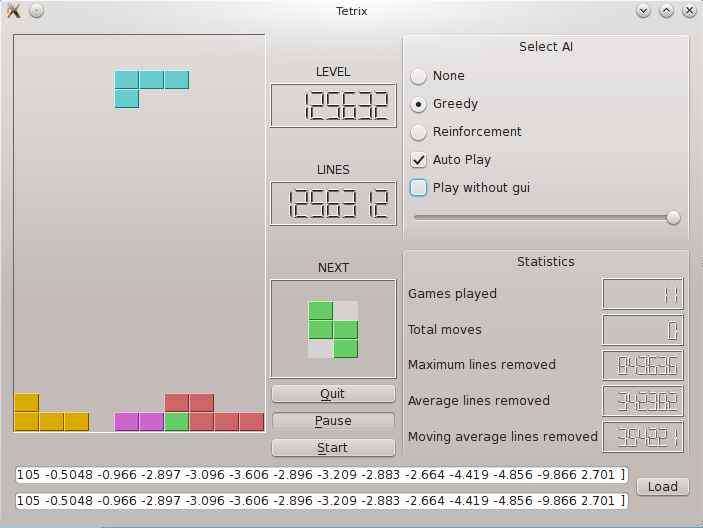
\includegraphics[width=0.5\textwidth]{img/three.png}
  \end{center}
  \vspace{-15pt}
  \caption{\footnotesize{The current number of removed lines already exceeds one million. Note, that the difference between the total and the moving average is not significant, as the game has been initiated with excellent weights, and the learning period was left out.}}
  \label{three}
  \vspace{-5pt}
\end{wrapfigure}

We also implemented an agent, which uses hardcoded rules to play Tetris. 
These rules are what we consider to be the ``naive'' way to play the game, comparable to an unexperienced player. 
The results of this rather unintelligent approach are used as a baseline. 
The algorithm with a learning function should by all means outperform the naive Agent.

We also use a greedy implementation, which simply uses given weights for the features to play the game, without learning from it. 
This is used to compare the quality of the learned weights (from the reinforcement learner implementation). 
These weights can simply be fed in through a text field in the GUI. 

\autoref{three} shows the greedy algorithm using obviously excellent values previously learned by the reinforcement learner.
The number of removed lines already exceeds 1,250,000 after 11 played games. 

\begin{wrapfigure}{r}{0.5\textwidth}
\vspace{-10pt}
  \begin{center}
    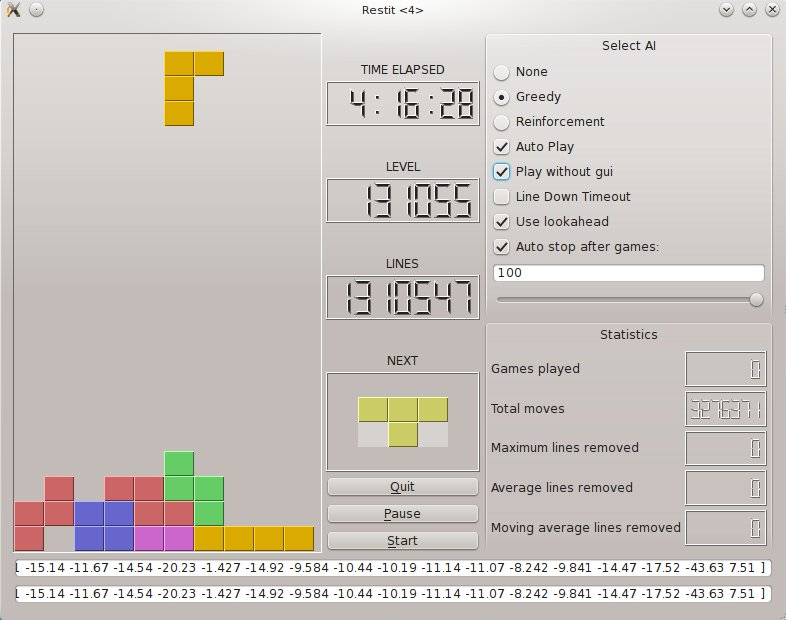
\includegraphics[width=0.5\textwidth]{img/restit4.jpg}
  \end{center}
  \vspace{-20pt}
  \caption{\footnotesize{More recent values: The greedy algorithm runs since more than four hours and has not lost one single game yet. The number of removed lines exceeds 1.3 million}}
  \label{four}
  \vspace{-15pt}
\end{wrapfigure}

The performance of the reinforcement learner usually does not outperform the greedy algorithm. 
To prevent getting stuck in a local maximum, the learner only chooses the ``best'' action (based on what it has learned before) to a certain probability. 
Otherwise, it just performs a random action, which can be interpreted as ``exploring'' new options without being too dependent on the possibly disadvantageous rules it has learned. 

The difference (exemplified with a rather old implementation of the reinforcement learner) can be seen in \autoref{four}.

Surprisingly, the weights learned by the reinforcement learner are actually worse when using lookahead compared to only using the current piece to determine the best action.
While the greedy agent, which just uses a given weight vector to play, improves using the lookahead, the reinforcement learner keeps on learning disadvantageous weights, which can, for example, result in stacking pieces on both edges of the board. 
Using a momentum adds to this effect.
We do not really have an explanation for this, so this might be a subject for further research.

What turned out to be the best strategy, was to let the agent run without lookahead, and then for the evaluation switch to a greedy method with lookahead using the learned weights.
We assume this is because the learned weights for tetris without lookahead approximate a desire for ``safe'' states.
Getting a high score only depends on staying alive for the longest possible amount of time, so essentially good weights when not using lookahead should approximate good weights when using lookahead.
It is much simpler for the learner to figure out what those weights are if lookahead is not enabled.

\begin{figure}[h!]
\centering
\begin{minipage}[t]{0.49\textwidth}
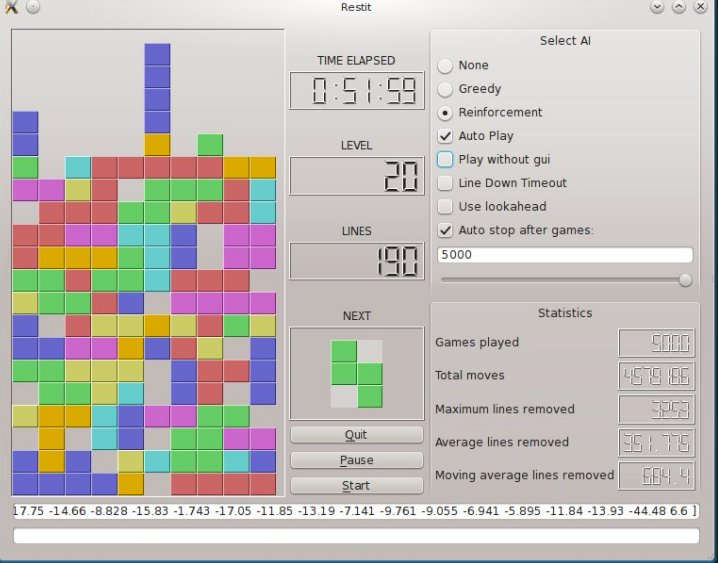
\includegraphics[width=\textwidth]{img/restit.jpg}
\end{minipage}
\begin{minipage}[t]{0.49\textwidth}
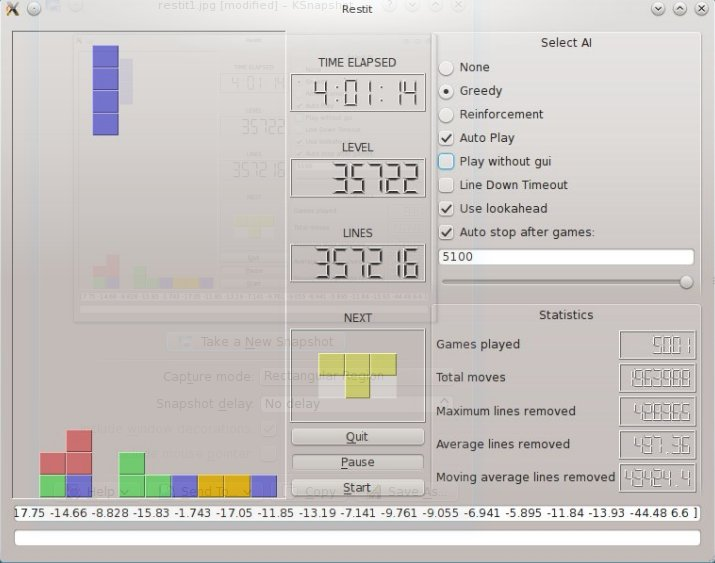
\includegraphics[width=\textwidth]{img/video1.jpg}
\end{minipage}
\caption{\footnotesize{The learner has played 5000 games in less than one hour, the greedy algorithm takes more than 3 hours for two games}}
\label{demo}
\end{figure}

We found empirically that a learning rate, $\alpha$, of 0.1 was suitable. A bigger learning rate seemed to cause the learned values to fluctuate.
On the other hand a lower learning rate caused the learning process to last unreasonably long. 
As \cite{zucker2009learning}, we found that a momentum, $\beta$, of 0.5 was suitable, as long as we don't use lookahead.

For the benchmark, we first let the learner run for 5000 games without using lookahead.
Then we switched off learning (greedy algorithm) and turned on lookahead for the evaluation and planned on running 100 games.
This is the same setup as \cite{zucker2009learning} used.
The problem however, was that the learner performed way better than we had expected. Just a single game usually lasts over two hours, and exceeds 600,000 removed lines.
This made it very impractical to do 100 tests. 

We ended up running 5 parallel learners, and tested them on just one game each. 
The results are shown in \autoref{resulttable}.

\begin{table}
\begin{center}
\begin{tabular}{|c|c|c|c|}
\hline 
Run & Lines removed in first game & Maximum Lines Removed & Games played\\ 
\hline 
1 & 336,989 & 630,468 & 6 \\ 
\hline 
2 & 659,616 & 659,616 & 1 \\ %J2 still running 2nd run at 611k+
\hline 
3 & 703,426 & 703,426 & 2 \\ %J1 141552 in second run, still running 3rd at  run at 334k
\hline 
4 & 1,700,103* & 1,700,103* & 1\\ 
\hline 
5 & 1,743,241* & 1,743,241* & 1\\ 
\hline 
\end{tabular}\\
\tiny{* interrupted before game ended} 
\end{center}

\caption{\footnotesize{5 different instances of the reinforcement learner trained with 5000 games each. Evaluated with learning turned off, using lookahead.}}
\label{resulttable}

\end{table}

%------------------------------------------------------------------------------

\section{Conclusions}
\label{conclusions}

With a few minor changes, we basically implemented the algorithm described by \cite{zucker2009learning}, but we surprisingly get much better results. 
We assume that training the weights without lookahead and only using it in the evaluation phase, makes a big difference. 
In general, we achieve better results than we expected and except for a few minor implementation bugs we consider this project as successful.
A video of the learning procedure can be found on YouTube\footnote{\href{http://www.youtube.com/watch?v=DXgtzFiRHdc}{Reinforcement Learner for Tetris Reloaded}}.


%------------------------------------------------------------------------------

%%%
% Sources
\bibliographystyle{agsm}
%\bibliographystyle{alphadin}
\bibliography{sources/sources}
\end{document}
